\documentclass[a4paper]{scrbook}
\usepackage{a4wide,amsmath,graphics}
\usepackage{hyperref}  %% need this for links and references in the document
\usepackage{array}     %% need this for more table formating (m{} and p{})
\usepackage{url}       %% support for URLs
\usepackage{float}     %% required for extra float placement
\usepackage{placeins}
\usepackage{subfig}
\usepackage{lscape}    %% landscape figures
\usepackage[disable]{todonotes}
\usepackage{color}
\usepackage[figuresright]{rotating}
\usepackage{minted}    %% excellent source code formating

\hypersetup{pdftitle={libpniio API review 2013 },
				pdfborder=0 0 0,
				colorlinks=false}

\setcapindent{0em}

\title{{\Huge{\tt libpnicore} Users Guide}}
\author{Eugen Wintersberger}

\newcommand{\libpnicore}{{\tt libpnicore}}
\newcommand{\sdarray}{{\tt static\_array}}
\newcommand{\darray}{{\tt dynamic\_array}}
\newcommand{\farray}{{\tt fixed\_dim\_array}}
\newcommand{\mdarray}{{\tt mdarray}}
\newcommand{\arrayview}{{\tt array\_view}}
\newcommand{\arrayerasure}{{\tt array}}
\newcommand{\numarray}{{\tt numeric\_array}}

\begin{document}
\maketitle
\tableofcontents
\chapter{Data types}
%%%documentation on data types

\FloatBarrier

\chapter{Arrays}
%%%documentation on arrays

C++ has no multidimensional array type (MDA) in its standard library. 
However, MDAs are crucial for the developmemt of scientific applications.
One of the reasons for the continuing success of languages like Fortran or Python
is their excellent support for MDAs\footnote{For Python arrays are introduced by
the {\tt numpy} package.}. The lack of an MDA type in C++
was indeed the spark that initiated the developement of \libpnicore.  Before
discussing \libpnicore s array facilities some terminology should be defined: 
%%%----------------------------------------------------------------------------
\begin{center}
\begin{tabular}{m{0.2\linewidth}p{0.7\linewidth}}
    element type (ET) &  referes to the data type of the individual elements
    stored in an MDA. For MDAs this will typically be a numeric type like an
    integer or a floating point number.\\

    rank $r$ & denotes the number of dimensions of an MDA \\

    shape $\mathbf{s}$ & is a vector of dimension $r$ whose elements are the
    number of elements along each dimension. The elements of $\mathbf{s}$ are
    denoted as $s_i$ with $i=0,\hdots,r-1$ \\
\end{tabular}
\end{center}
%%%----------------------------------------------------------------------------
The hart of \libpnicore's MDA support is the {\tt mdarray} template. 
{\tt mdarray} is extremely powerfull. Thus, using {\tt mdarray} directly to
define array types is not for the faint harted.  To simplify
the usage of multidimensional arrays the library provides three templates
derived form {\tt mdarray} which are easy to use.  
%%%----------------------------------------------------------------------------
\begin{center}
\begin{tabular}{m{0.2\linewidth}p{0.7\linewidth}}
\sdarray &  
a static arrays whose shape, rank, and element type are fixed at compile time.
\\
\farray &
element type and rank are fixed at compile time but the shape can be changed at
runtime. \\
\darray & 
a fully dynamic array type where only the element type must be known at compile
time. The rank as well as the shape can be altered at runtime\\
\end{tabular}
\end{center}
%%%----------------------------------------------------------------------------
These types are all defined in {\tt pni/core/arrays.hpp}.
In addition to this two basic templates there are several utility classes and
templates like
%%%----------------------------------------------------------------------------
\begin{center}
\begin{tabular}{m{0.15\linewidth}p{0.7\linewidth}}
\arrayview &  a template providing a particular view on an array (see
Sec.~\ref{sec:array:array_slicing}) \\
\arrayerasure & a type erasure that can be used with any instance of an array
template (see Chapter~\ref{chapter:type_erasure})
\end{tabular}
\end{center}
%%%----------------------------------------------------------------------------

All array types derived from {\tt mdarray} provide the following features
\begin{enumerate}
\item unary and binary arithmetics if the element type is a numeric type.
\item slicing to extract only a part of a large array
\item simple access to data elements using variadic operators.
\item all array types are full STL compliant containers and thus can be used
along with STL algorithms.
\end{enumerate}

\section{Array construction and inquery}
    
Constructing arrays is rather simple by means of the {\tt ::create} function
provided by the array templates. The next example shows how to create arrays 
using this static function

\inputminted[fontsize=\small,linenos,firstline=24,frame=lines]{cpp}
{../examples/array_create.cpp}
In line $12$ a concrete array type is defined from the {\tt dynamic\_array}
utility template.
The {\tt::create} function comes in three flavors as shown in the previous
example
\begin{description}
\item[line 17] it takes the shape of the array as a container and constructs the
array from this. In this case the storage container is allocated internally. 
\item[line 20] the storage container is passed along with the shape.
\item[line 24] here the shape and the container are passed as initializer lists
- this can make the syntax more readable in some cases.
\end{description}
After an array has been created we may want to retrieve some of its basic
properties. In the next example we do exactly this 

\inputminted[fontsize=\small,linenos,firstline=24,frame=lines]{cpp}
{../examples/array_inquery.cpp}
The important part is the implementation of the {\tt show\_info} function
template starting at line $14$. The function template {\tt type\_id} is used in
line $17$ to retrieve the type ID of the arrays element type. {\tt rank} in line
$18$ returns the number of dimension and {\tt size} in line $23$ the total
number of elements stored in the array. 
The {\tt shape} template function in line $20$ returns the number of elements
along each dimension stored in a user provided container type.

The content of arrays can be copied to and from containers using the standard 
{\tt std::copy} template function from the STL. In addition a version of the
assignment operator is provided which allows assignment of values from an
initializer list. This is particularly useful for static arrays which basically
do not require construction. 
\begin{minted}[fontsize=\small,linenos,frame=lines]{cpp}
typedef .... static_array_type; 

static_array_type a;

a = {1,2,3,4,5};
\end{minted}

\section{Linear access to data}
As already mentioned in the first section of this chapter, the array types
provided by \libpnicore\ are fully STL compliant containers. They provided all
the iterators required by the STL. 
Before we have a look on STL lets first investigate how to simply access data
elements in an array

\inputminted[fontsize=\small,linenos,firstline=24,frame=lines]{cpp}
{../examples/array_linear_access.cpp}
For all array types the new C++ {\em for-each} construction can be used as shown
in lines $24$ and $34$. Unchecked access (no index bounds are checked) is
provided via the {\tt []} operator as demonstrated in line $27$. Finally, in
cases where the index should be checked use the {\tt at()} method like in lines 
$30$ and $31$.
Some of the operations in this example can be done much more efficient with STL
algorithms as demonstrated in the next example

\inputminted[fontsize=\small,linenos,firstline=24,frame=lines]{cpp}
{../examples/array_stl.cpp}
In line $19$ {\tt std::fill} is used to initialize the array to $0$ and 
{\tt std::generate} in line $25$ fills it with random numbers using a lambda
expression . The rest of the example should be trivial (if not, please lookup a
good C++ STL reference).

\section{Multidimensional access}

Though being an important feature, linear access to multidimensional arrays is
not always useful. In particular the last example where we pretended to work on
image data implementing algorithms would be rather tedious if we would have had
only linear access. It is natural for such objects to think in pixel coordinates
$(i,j)$ rather than the linear offset in memory. 
\libpnicore\ provides easy multidimensional access to the data stored in an
array. The next example shows how to use this feature to work only on a small
region of the image data as defined in the last example
\inputminted[fontsize=\small,linenos,firstline=24,frame=lines]{cpp}
{../examples/array_multiindex.cpp}
The interesting part here are lines $36$ and $37$. You can pass the
multidimensional indexes either as a variadic argument list to the  {\tt ()}
operator of the array type (as in line $36$) or you can use a container like 
in line $37$. The former approach might look a bit more familiar, however, in
some cases when decisions have to made at runtime the container approach might
fits better. However, passing containers reduces access performance
approximately by a factor of 2. Thus, as a rule of thumb you should always use
the variadic form when you know the number of dimensions the array has and
containers only in those cases where this information is only available at
runtime.

\section{Array views and slicing}

In the previous example multiindex access was used to do work on only a small
part of the image data. \libpnicore\ provides view types for arrays which would
make these operations easier. Views are created by passing instances of {\tt
slice} to the {\tt ()} operator of an array type. Slices in \libpnicore\ work
pretty much the same as in python. Lets have a look on the following example
\inputminted[fontsize=\small,linenos,firstline=24,frame=lines]{cpp}
{../examples/array_view.cpp}
The view is created in line $30$ where the slices are passed instead of integer
indices to the {\tt ()} operator. A slice selects an entire index range along a
dimension. The first argument to the {\tt slice} constructor is the starting
index and the last the stop index of the range. The stop index is not included
(just as it is the case with Python slices). If the {\tt ()} operator of an
array is called with any of its arguments being a slice a view object is
returned instead of a single value or reference to a single value. 
View objects are pretty much like arrays themselves. However, they do not hold
data by themselves but only a reference to the original array. 
Like arrays they are fully STL compliant containers and thus can be used with
STL algorithms as shown in lines $31$ and $33$. 

View types can be copied and moved and thus can be stored in STL containers as
shown in the next example
\inputminted[fontsize=\small,linenos,firstline=24,frame=lines]{cpp}
{../examples/array_view_container.cpp}
Here we apply the algorithms from the previous example not to a single but to
several selections in the image. As shown in lines $32$ to $34$ we can safely
store views in a container and later iterate over it.

In general views make algorithm development much easier as we have to develop
algorithms only for entire arrays. If it should be applied to only a part of an
array we can use a view and pass it to the algorithm. As views expose the same
interface as an array the algorithm should work on views too.

\section{Arithmetic expressions}

Array and view types fully support the common arithmetic
operators {\tt +}, {\tt *}, {\tt /}, and {\tt -} in their binary and unary
forms. The binary versions are implemented as expression templates avoiding the
allocation of unnecessary temporary and giving the compiler more possibilities
to optimize the code. 
Views, arrays and scalars can be mixed within all arithmetic expressions. 
There is nothing magical with expression templates as they work entirely
transparent to the user. Just use the arithmetic expressions as you are used to
\inputminted[fontsize=\small,linenos,firstline=24,frame=lines]{cpp}
{../examples/array_arithmetic1.cpp}
The important line here is $24$ where arrays and scalars are mixed in an
arithmetic expression.
One can also mix arrays, selections, and scalars as the next examples 
shows
\inputminted[fontsize=\small,linenos,firstline=24,frame=lines]{cpp}
{../examples/array_arithmetic2.cpp}
In line $30$ a single image frame is selected from a stack of images and used in
line $31$ in an arithmetic expression. In fact, what we are doing here is,
we are writing the corrected data back on the stack since {\tt curr\_frame} is
just a view on the particular image in the stack.

\section{Some more elaborate example}
\subsection{Matrix-vector multiplications}
In the last example matrix vector multiplications are treated. The full code can
be viewed in {\tt array\_arithmetic3.cpp} in the source distribution. But lets
first start with the header
\inputminted[fontsize=\small,linenos,firstline=24,lastline=39,firstnumber=24,frame=lines]{cpp}
{../examples/array_arithmetic3.cpp}
Besides including all required header files matrix and vector templates are 
defined in lines $37$ and $38$ using the new C++11 template aliasing.

\inputminted[fontsize=\small,linenos,firstline=40,lastline=63,firstnumber=40,frame=lines]{cpp}
{../examples/array_arithmetic3.cpp}
In lines $42$ and $57$ output operators are defined for vectors and matrices.
These will allow us to write the data to a stream. 


The implementation of the matrix vector multiplication is shown in the next
block. In other words
\begin{align}
 \mathbf{r} = A\mathbf{v} \mbox{ or } r_j = A_{j,i}v_i
\end{align}
with $A$ denoting a $N\times N$ matrix and $\mathbf{r}$ and $\mathbf{v}$ are
$N$-dimensional vectors. In all formulas Einsteins sum convention is used.
\inputminted[fontsize=\small,linenos,firstline=64,lastline=80,firstnumber=64,frame=lines]{cpp}
{../examples/array_arithmetic3.cpp}
In line $74$ we select the $i$-th row of the matrix and compute the inner
product of the row vector and the input vector in line $75$. 
The vector matrix multiplication
\begin{align}
 \mathbf{r} = \mathbf{v}A\mbox{ or } r_i = v_j A_{j,i}
\end{align}
is computed analogously 
\inputminted[fontsize=\small,linenos,firstline=80,lastline=95,firstnumber=80,frame=lines]{cpp}
{../examples/array_arithmetic3.cpp}
despite the fact that we are choosing the appropriate column instead of a row in 
line $90$. Finally we need an implementation for the matrix - matrix
multiplication
\begin{align}
C = AB \mbox{ or } C_{i,j} = A_{i,k}B_{k,j}
\end{align}
\inputminted[fontsize=\small,linenos,firstline=96,lastline=115,firstnumber=96,frame=lines]{cpp}
{../examples/array_arithmetic3.cpp}
The rows and columns are selected in lines $107$ and $108$ respectively. 
Line $109$ finally computes the inner product of the row and column vector.

Finally the main program shows a simple application of these template functions. 
\inputminted[fontsize=\small,linenos,firstline=116,lastline=138,firstnumber=116,frame=lines]{cpp}
{../examples/array_arithmetic3.cpp}
It is important to understand that the appropriate function is determined by the
types of the arguments (vector or matrix). This is a rather nice example of how
to use the typing system of C++ to add meaning to objects.

\FloatBarrier

\chapter{Program configuration utilities}
%%% some documentation on the configuration facility 

One of the most tedious tasks when writing applications is how to handle its
configuration. There are several possibilities how a user can tell a program
about input arguments and parameters 
\begin{itemize}
\item via command line options and arguments
\item via environment variables of the calling shell
\item and via configuration files.
\end{itemize}
It is important to note that this is information the program has only read-only
access too. \libpnicore\ provides some simple functions to make programs aware
of command line options and arguments as well as of configuration files. The
facility provided by \libpnicore\ is based on the \texttt{boost::program\_options}
library. However, its interface is much easier to use.  
What makes this facility so interesting for scientific applications is the fact
that every option or argument can be given a distinct data type. 

\section{Command line options and arguments}

One possibility to provide information to a program is by means of command line
arguments and options which are passed to the program when called from a shell
by the user. This is particularly true for Unix systems where many programs are
called via the command line rather than via a Desktop. 

In this section we will deal with all the basics required to use \libpnicore s
configuration facilities. Read this in any case even if you only want to use a
configuration file as many of the things written is true also for configuration
files. 

\subsection{Unix conventions}


In the Unix world we have to distinguish between command line {\em arguments}
and {\em options}. The former ones are strings which can typically appear
anywhere in the command calling the program from the shell. The meaning of a
particular option depends only on its position within the command used to run a
program. 
The latter ones, {\em options}, are introduced by special tokens in the calling
command. This token determines the meaning of a particular option. Thus options
can appear in any order after the name of the program. 
To get a better feeling about arguments and options lets have a look on a
typical command line call on a Unix or Linux system
\begin{minted}{ps1}
> program -oresult.dat --wavelength=1.234 in1.dat in2.dat in3.dat
\end{minted}
The three input files at the end of the call (\texttt{in1.dat}, \texttt{in2.dat}, and
\texttt{in3.dat}) are passed as arguments. They can appear in any order and there
is no way to distinguish one from the other and will be processed in the order
of their appearance. This is in contrast to \texttt{result.dat} and \texttt{1.234}
which are passed as options. An option can be identified by a {\em short name} (by
convention this must be a single character) as it is the case for \texttt{
result.dat} or by a {\em long name}, like for \texttt{1.234}, which must be a
string without whitespaces. Short names are are introduced by a single '\texttt{-}'
and followed immediately by the value of the option. Long names start with
'\texttt{--}' followed by a '\texttt{=}' and the value of the option. An option can have both,
a long and a short name. While short names are typically used when a program is
called interactively by a user to minimize the typing effort, long names are
mostly used when a program is called from a script. As they are not limited to a
single character long names can be chosen much more descriptive than short
names. Being restricted to a single character short names are sometimes only
used for options which are frequently used in interactive calls while scarcely
used options have only a long name.

\subsection{Creating a simple program configuration}

Creating a configuration for a program involves three classes
\begin{itemize}
\item \texttt{configuration} which, in the end, will hold the configuration data
and provide access to it
\item \texttt{config\_option} describing a single command line option
\item \texttt{config\_argument} which we will use to describe command line arguments 
\end{itemize}
Lets start with the above example. The source code of the program would maybe
look like this

\begin{minted}{cpp}
#include <vector>
#include <pni/core/types.hpp>
#include <pni/core/config/configuration.hpp>
#include <pni/core/config/config_parser.hpp>

using namespace pni::core;

typedef std::vector<string> input_files;

int main(int argc,char **argv)
{
    configuration config;
    config.add_option(config_option<string>("output","o","output file"));
    config.add_option(config_option<float64>("wavelength","w"));
    config.add_argument(config_argument<input_files>("input",-1));

    parse(config,cliargs2vector(argc,argv));

    return 0;
}
\end{minted}

\section{Configuration files}

Configuration files handled by \libpnicore\ follow the \texttt{INI}-file syntax as
used by Windows. 
An example file would look like this
\begin{minted}{ini}
#experiment.cfg
[beam]
wavelength = 1.543
divergence = 0.12
diameter   = 1.23

[sample]
name = sample1
description = first sample in the series
\end{minted}
To read this file create the following configuration in the program
\begin{minted}{cpp}
#include <pni/core/types.hpp>
#include <pni/core/configuration.hpp>
#include <pni/core/config_parser.hpp>

using namespace pni::core;

int main(int argc,char **argv)
{
    configuration config;

    config.add_option(config_option<float64>("beam.wavelength",""));
    config.add_option(config_option<float64>("beam.divergence",""));
    config.add_option(config_option<float64>("beam.diameter",""));
    config.add_option(config_option<string>("sample.name",""));
    config.add_option(config_option<string>("sample.description",""));

    parse(config,"experiment.cfg");

    //use the options
}
\end{minted}


\section{Using configuration files and command line options together}


\FloatBarrier

\chapter{Benchmark utilities}
\FloatBarrier

\appendix
\chapter{Some internals on multidimensional arrays}
One of the major motivations for the development of \libpnicore\ was the lack of
native support for multidimensional (MD) arrays in C++. This section goes into
details how such arrays are implemented in \libpnicore. Thus this part of the
documentation is intended for developers and those who want to know more about
the internals of \libpnicore. 

The classical approach towards MD arrays in C/C++ would be to do something like
this
\begin{minted}{cpp}
double matrix[3][3];
\end{minted}
However, this approach has a whole bunch of problems
\begin{enumerate}
\item the variable {\tt matrix} is allocated on the stack which will cause
problems if the matrix becomes large
\item there is no easy way how to allocate such a variable on the heap (at least
not at runtime)
\item there is no native support for arithmetic operations on multidimensional
arrays 
\item there is no native support for slicing (select a sub region) of such
arrays.
\end{enumerate}
There is a language that has perfect support for MD arrays: Fortran. In the
standards Fortran 90 and higher the language shows all the features required to
easily work with MD arrays. It is thus not surprising that Fortran was an
inspiration for the design of the MD array interface in \libpnicore. 
There is still one question left: if Fortran is so superior with MD arrays, why
not write the numerical part of the software in Fortran and everything else in
C++? The reason is simple: while Fortran is quite good for writing short and
rather straight forward numerical applications, its lack of a standard library
providing higher level data structures such as lists or maps render it
inconvenient for the implementation of large software systems. In addition, its
lack of {\em generics} or {\em template} support requires a user to reimplement
an algorithm for each desired data type which is obviously horribly inefficient. 
C++ offers all the tools for implementing a fast and easy to use MD array
interface whose performance can compete with those of Fortran as will be shown
later. 

\section{Basic concepts of multidimensional arrays}

Lets start with a definition of terms:
\begin{description}
\item[rank] the number of dimensions of an MD array, typically abbreviated with
$r$
\item[elements per dimension] the number of elements along each dimension is
denoted by $n_i$ where $i=1,\hdots,r$.
\item[total number of elements] denoted by $n_{\mathrm{tot}}$ is the total
number of elements stored in a MD array and can be computed with 
\begin{align}
    n_{\mathrm{tot}} = \prod_{i=1}^r n_i
\end{align}
\item[element type] the data type of the elements stored in the array,
abbreviated with {\tt ETYPE}. 
\end{description}

%%-----------------------------------------------------------------------------
\begin{figure}[tb]
\centering
\begin{minipage}[c]{0.55\linewidth}
\centering
\resizebox{\linewidth}{!}{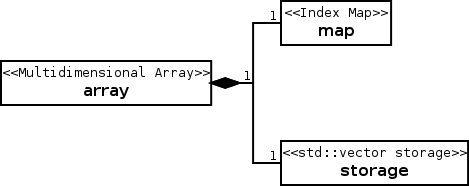
\includegraphics{pics/md_array_basic_structure.png}}
\end{minipage}
\hfill
\begin{minipage}[c]{0.39\linewidth}
\caption{{\small\label{fig:array_app:basic_structure} A MD array consists of a
storage and an index map. The former holds all the data elements in memory while
the latter one maps multidimensional indexes uniquely to linear offsets in the
storage.
}}
%%-----------------------------------------------------------------------------
\end{minipage}
\end{figure}
To overcome the issues that classical MD arrays have in C or C++ we need a more
elaborate data structure to describe the array. In \libpnicore\ a MD array
consists of two components (see also Fig.~\ref{fig:array_app:basic_structure})
\begin{enumerate}
\item a linear storage of size $n_{\mathrm{tot}}$ for elements of type {\tt
ETYPE}
\item a so called index map {\tt IMAP} which is a data structure providing a
unique mapping between a multidimensional index $(i,j,k,\hdots)$ and a linear
offset in the storage. 
\end{enumerate}
The storage can be any data structure that can hold elements of type {\tt ETYPE}
contiguously in memory and exposes an interface compatible to that of {\tt std::vector}.

\section{Index maps}

%%%----------------------------------------------------------------------------
\begin{figure}[tb]
\centering
\begin{minipage}{0.3\linewidth}
\centering
\resizebox{\linewidth}{!}{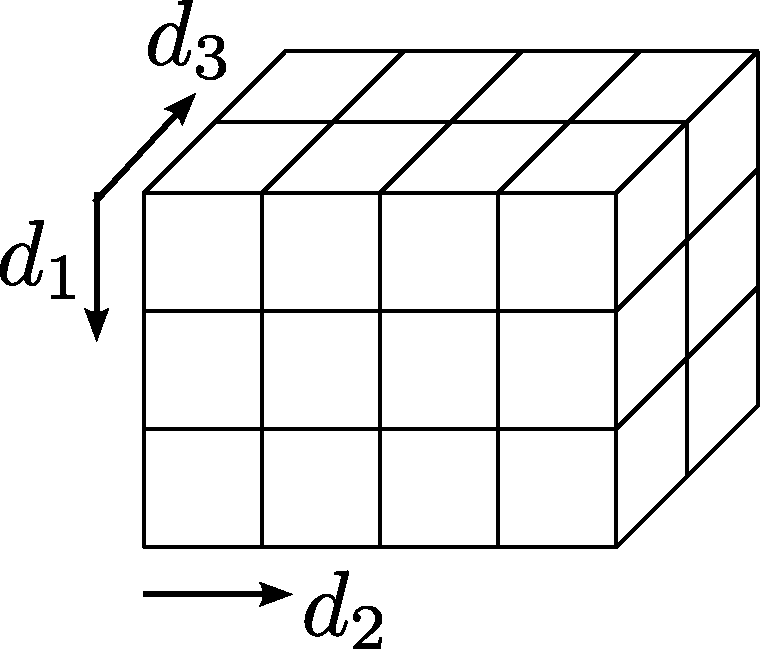
\includegraphics{pics/array_3d.pdf}}
\end{minipage}
\hfill
\begin{minipage}{0.45\linewidth}
\caption{{\small\label{fig:array_app:array_3d}
The 3-dimensional array of shape $(3,4,2)$ which will be used for all following
examples. 
}}
\end{minipage}
\end{figure}
%%%----------------------------------------------------------------------------
Index maps serve two purposes 
\begin{enumerate}
\item compute the linear offset for a given multidimensional index
\item compute the multidimensional index for a given offset.
\end{enumerate}
It is indeed the implementation of the index map which determines whether or not
an array is in row- or column-major ordering (see also
sections~\ref{sec:c_ordering} and \ref{sec:f_ordering} for details on this).
When an element of a MD array is addressed by a multidimensional index
$(i,j,k,\hdots)$ this index must be converted (uniquely) to a linear offset in
the storage. There are currently two standard schemas how MD indexes are mapped
to linear memory
\begin{itemize}
\item {\em row-major ordering} (this is how all C-like languages are doing it) where
the last index varies fastest and is thus continuous in memory
\item and {\em column-major ordering} (the Fortran way) where the first index
varies fastest and is thus continuous in memory.
\end{itemize}

In more general terms the question reads: which index varies fastest or which
index is contiguous in memory. In row-major this is true for the last index
while for column-major ordering the first index is contiguous in memory.
These two cases will be now discussed in more detail.

For all further considerations we will use an example as depicted in
Fig.~\ref{fig:array_app:array_3d} which is a 3 dimensional array of arbitrary
element type and shape $(3,4,2)$.

\subsection{Row major- or C-ordering}\label{sec:c_ordering}

%%-----------------------------------------------------------------------------
\begin{figure}[tb]
\centering
\begin{minipage}{0.45\linewidth}
\centering
\resizebox{\linewidth}{!}{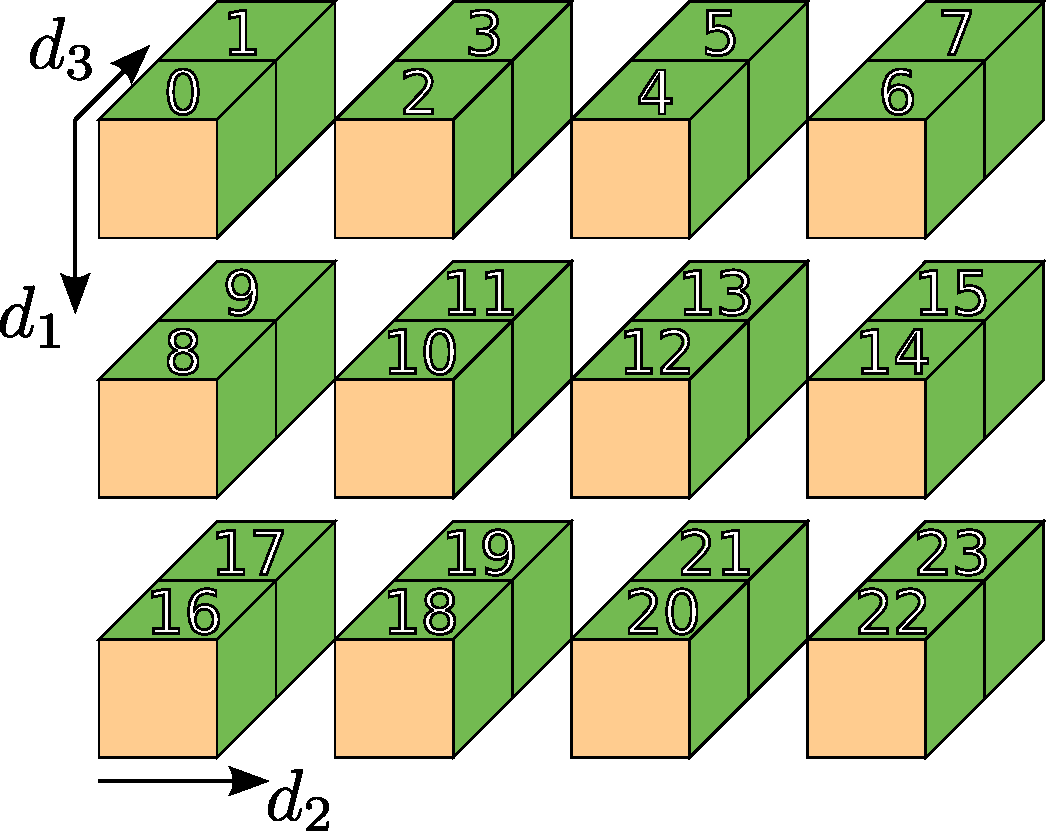
\includegraphics{pics/array_3d_corder.pdf}}
\end{minipage}
\hfill
\begin{minipage}{0.4\linewidth}
\caption{{\small\label{fig:array_app:array_3d_corder}
The array shown in Fig.~\ref{fig:array_app:array_3d} in C-ordering (row major
ordering). The last index varies fastest and is thus contiguous in memory. 
}}
\end{minipage}
\end{figure}
%%-----------------------------------------------------------------------------
Row major ordering is the standard layout in memory for multidimensional array
sin C and most other languages derived from it. In this case the last index
varies fastest and is thus contiguous in memory as shown in
Fig.~\ref{fig:array_app:array_3d_corder}. 
The transformation of the MD index $\mathbf{i}=(i,j,k)$ to the linear offset 
$o$ can be written as a scalar product 
\begin{align}\label{eq:array_app:offset_formula}
    o = \mathbf{s}\mathbf{i}
\end{align}
where $\mathbf{s}$ denotes the stride vector whose elements are given with
\begin{align}
    s_i &= \prod_{j=i+1}^r n_j \\
    s_r &= 1
\end{align}
For the above example the stride vector would read $\mathbf{s}=(8,2,1)$. 
The other direction, computing the index from a given offset is a bit more
difficult. 

\subsection{Column major- or Fortran-ordering}\label{sec:f_ordering}
%%-----------------------------------------------------------------------------
\begin{figure}[tb]
\centering
\begin{minipage}{0.5\linewidth}
\centering
\resizebox{\linewidth}{!}{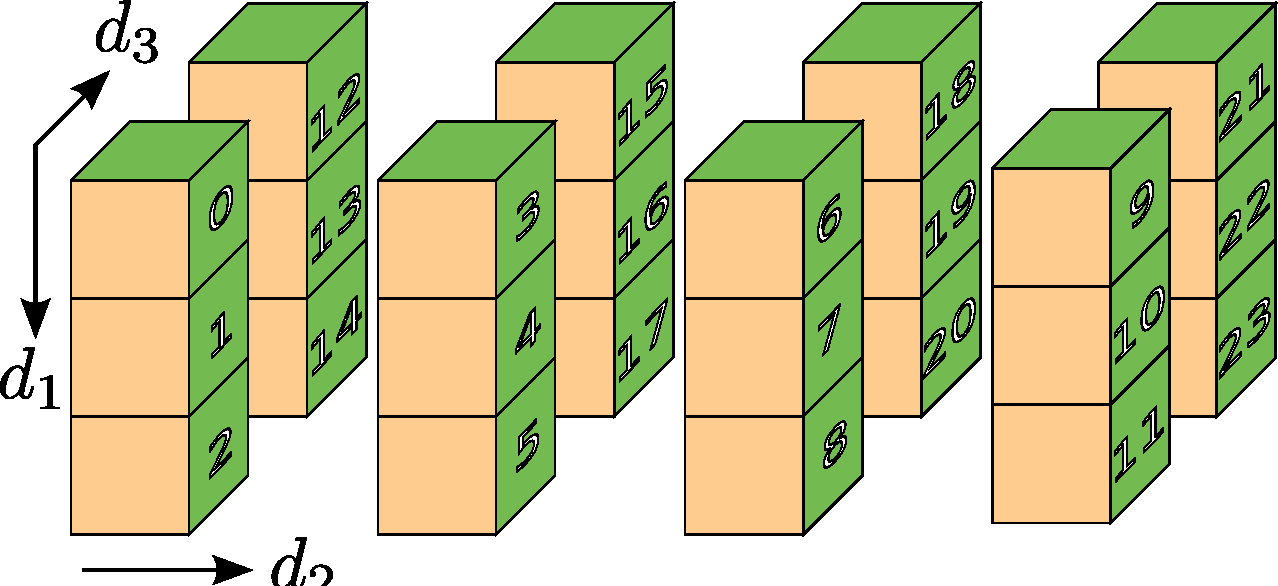
\includegraphics{pics/array_3d_forder.pdf}}
\end{minipage}
\hfill
\begin{minipage}{0.4\linewidth}
\caption{{\small\label{fig:array_app:array_3d_forder}
The array shown in Fig.~\ref{fig:array_app:array_3d} in Fortran-ordering (column major
ordering). The first index varies fastest and is thus contiguous in memory. 
}}
\end{minipage}
\end{figure}
%%-----------------------------------------------------------------------------
This schema for data organization is commonly used in languages like Fortran,
Pascal, or Ada. The layout of data elements in memory for our example array is
shown in Fig.~\ref{fig:array_app:array_3d_forder}. The formula for the offset
calculation is the same as for C-ordering and can be found  in
Eq.~(\ref{eq:array_app:offset_formula}). What is different here is the stride
vector. The algorithm to compute its elements reads
\begin{align}
    s_0 &= 1 \\
    s_i &= \prod_{j=0}^in_j
\end{align}

\subsection{Arbitrary ordering}\label{sec:a_ordering}
%%-----------------------------------------------------------------------------
\begin{figure}[tb]
\centering
\begin{minipage}{0.35\linewidth}
\centering
\resizebox{\linewidth}{!}{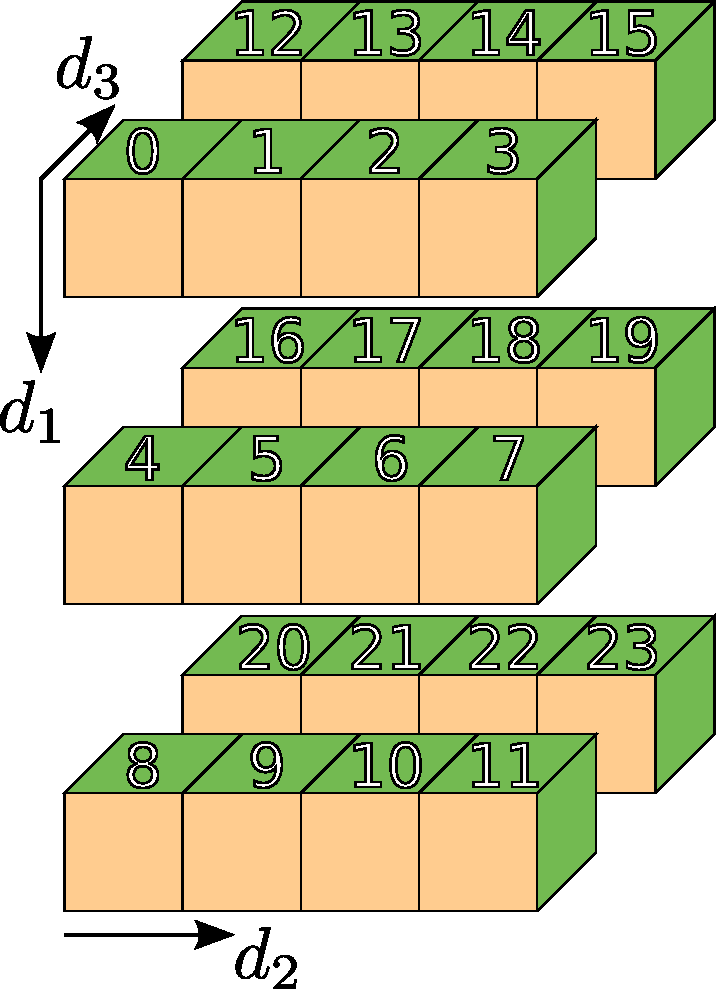
\includegraphics{pics/array_3d_aorder.pdf}}
\end{minipage}
\hfill
\begin{minipage}{0.4\linewidth}
\caption{{\small\label{fig:array_app:array_3d_aorder}
The array shown in Fig.~\ref{fig:array_app:array_3d} using an arbitrary ordering
scheme where the second index varies fastest, followed by the first and the
last.
}}
\end{minipage}
\end{figure}
%%-----------------------------------------------------------------------------

\subsection{Index maps in \libpnicore}

After having discussed now all the theoretical background about index maps lets
have a look how these objects are implemented in \libpnicore.

\subsubsection{Classes and their relationships}

\begin{figure}[tb]
\centering
\begin{minipage}[c]{0.49\linewidth}
\centering
\resizebox{\linewidth}{!}{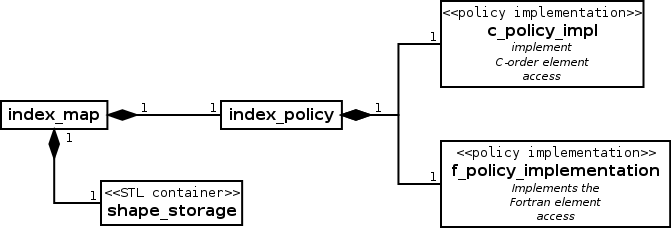
\includegraphics{pics/index_map_diagram.png}}
\caption{{\small\label{fig:array_app:index_map_diagram}
An ordinary index map consists of an instance of {\tt index\_policy}
(transforming indexes to offsets and vice verse) and a
storage for the number of elements along each dimension. 
}}
\end{minipage}
\hfill
\begin{minipage}[c]{0.49\linewidth}
\centering
\resizebox{\linewidth}{!}{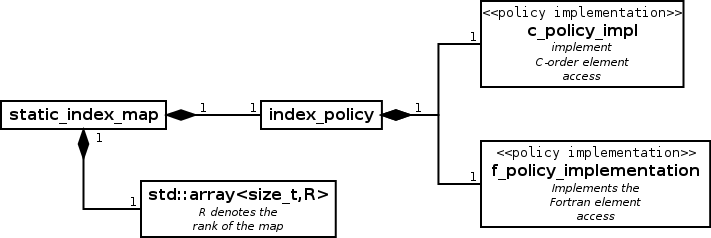
\includegraphics{pics/static_index_map_diagram.png}}
\caption{{\small\label{fig:array_app:static_index_map_diagram}
Static index maps have a static storage whose content cannot be altered. They
are entirely defined at compile time.
}}
\end{minipage}
\end{figure}
There are two fundamental templates for index maps available: {\tt index\_map}
and {\tt static\_index\_map}. The former one can be used to for general index
maps while the latter one considers the special case for a static index map
for which the rank and the number of elements along each dimension are fixed at
compile time. 

\subsubsection{The basic interface}

\begin{minted}{cpp}
class index_map
{
    public:
    //======================public types========================
    typedef .... const_iterator;

    //======================public methods======================
    index_map();                  //default constructible
    index_map(const index_map &); //copy constructible 

    index_map &operator=(const index_map &s); //copy assignable 

    //compute offset from a varidic list of indexes
    template<typename ...ITYPES> size_t offset(ITYPES ...indices);

    //compute offset from a container type
    template<CTYPE> size_t offset(const CTYPE &v);

    //compute index from a given offset
    template<CTYPE> CTYPE index(size_t offset);

    size_t rank() const;  //get number of dimensions
    size_t size() const;  //get number of dimensions
    
    const_iterator begin() const; 
    const_iterator end() const; 

};
\end{minted}

\section{Selections}

\section{Array arithmetics}

\section{Performance considerations}


\FloatBarrier

\end{document}
